\documentclass[a4paper,11pt,fleqn,dvipsnames,twoside,openright]{memoir} 	% Openright aabner kapitler paa hoejresider (openany begge)

%%%% PACKAGES %%%%

% ¤¤ Oversaettelse og tegnsaetning ¤¤ %
\usepackage[utf8]{inputenc}					% Input-indkodning af tegnsaet (UTF8)
\usepackage[danish]{babel}					% Dokumentets sprog
\usepackage[T1]{fontenc}					% Output-indkodning af tegnsaet (T1)
\usepackage{ragged2e,anyfontsize}			% Justering af elementer
\usepackage{fixltx2e}						% Retter forskellige fejl i LaTeX-kernen

																			
% ¤¤ Figurer og tabeller (floats) ¤¤ %
\usepackage{graphicx} 						% Haandtering af eksterne billeder (JPG, PNG, EPS, PDF)
%\usepackage{eso-pic}						% Tilfoej billedekommandoer paa hver side
%\usepackage{wrapfig}						% Indsaettelse af figurer omsvoebt af tekst. \begin{wrapfigure}{Placering}{Stoerrelse}
\usepackage[space]{grffile}					% Bør gøre det muligt at have mellemrum i filnavne.
\usepackage{multirow}                		% Fletning af raekker og kolonner (\multicolumn og \multirow)
\usepackage{multicol}         	        	% Muliggoer output i spalter
\usepackage{rotating}						% Rotation af tekst med \begin{sideways}...\end{sideways}
\usepackage{colortbl} 						% Farver i tabeller (fx \columncolor og \rowcolor)
\usepackage[usenames,dvipsnames]{xcolor}	% Definer farver med \definecolor. Se mere: http://en.wikibooks.org/wiki/LaTeX/Colors
%\usepackage{flafter}						% Soerger for at floats ikke optraeder i teksten foer deres reference
\let\newfloat\relax 						% Justering mellem float-pakken og memoir
\usepackage{float}							% Muliggoer eksakt placering af floats, f.eks. \begin{figure}[H]
\setlength{\heavyrulewidth}{0.15em}			% Sætter \toprule og \bottomrule til fast størrelse (0.08 er default)
%\setlength{\lightrulewidth}{0.05em}		% Sætter \midrule til fast størrelse (0.05 er default)
\usepackage{array}							% Bruges i forbindelse med \newcolumntype-command under egne commands
\usepackage{pdfpages}						% Bruges så der kan indsættes pdf, som sider (se forside for eksempel)
\usepackage{tablefootnote}


% ¤¤ Matematik mm. ¤¤
\usepackage{amsmath,amssymb,stmaryrd} 		% Avancerede matematik-udvidelser
\usepackage{mathtools}						% Andre matematik- og tegnudvidelser
\usepackage{textcomp}                 		% Symbol-udvidelser (f.eks. promille-tegn med \textperthousand )
\usepackage{rsphrase}						% Kemi-pakke til RS-saetninger, f.eks. \rsphrase{R1}
\usepackage[version=3]{mhchem} 				% Kemi-pakke til flot og let notation af formler, f.eks. \ce{Fe2O3}
\usepackage{siunitx}						% Flot og konsistent praesentation af tal og enheder med \si{enhed} og \SI{tal}{enhed}
\sisetup{locale=DE}							% Opsaetning af \SI (DE for komma som decimalseparator) 

% ¤¤ Referencer og kilder ¤¤ %
\usepackage[danish]{varioref}				% Muliggoer bl.a. krydshenvisninger med sidetal (\vref)
\usepackage{natbib}							% Udvidelse med naturvidenskabelige citationsmodeller
\usepackage{xr-hyper}							% Referencer til eksternt dokument med \externaldocument{<NAVN>}
\externaldocument[DokRap-]{../Dokumentationsrapport/Dokumentationsrapport}	% Muliggør eksterne referencer til produktrapporten
%\usepackage{glossaries}					% Terminologi- eller symbolliste (se mere i Daleifs Latex-bog)



% ¤¤ Misc. ¤¤ %
\usepackage{lipsum}							% Dummy text \lipsum[..]
\usepackage[shortlabels]{enumitem}			% Muliggoer enkelt konfiguration af lister
\usepackage{pdfpages}						% Goer det muligt at inkludere pdf-dokumenter med kommandoen \includepdf[pages={x-y}]{fil.pdf}	
\pdfoptionpdfminorversion=6					% Muliggoer inkludering af pdf dokumenter, af version 1.6 og hoejere
\pretolerance=2500 							% Justering af afstand mellem ord (hoejt tal, mindre orddeling og mere luft mellem ord)

% Kommentarer og rettelser med \fxnote. Med 'final' i stedet for 'draft' udloeser hver note en error i den faerdige rapport.
\usepackage[footnote,draft,danish,silent,nomargin]{fixme}		


%%%% CUSTOM SETTINGS %%%%

% ¤¤ Marginer ¤¤ %
\setlrmarginsandblock{3.5cm}{2.5cm}{*}		% \setlrmarginsandblock{Indbinding}{Kant}{Ratio}
\setulmarginsandblock{2.5cm}{3.0cm}{*}		% \setulmarginsandblock{Top}{Bund}{Ratio}
\checkandfixthelayout 						% Oversaetter vaerdier til brug for andre pakker

%	¤¤ Afsnitsformatering ¤¤ %
\setlength{\parindent}{0mm}           		% Stoerrelse af indryk
\setlength{\parskip}{3mm}          			% Afstand mellem afsnit ved brug af double Enter
\linespread{1,1}							% Linie afstand
\newcommand{\tab}{\hspace*{2em}}			% ved \tab{} indrykkes det i klammerne ind
\usepackage{titlesec}							%Muliiggøre ændring af sections i alle lag
\titleformat*{\section}{\LARGE\bfseries\color{NavyBlue}}		%section = størst
\titleformat*{\subsection}{\Large\bfseries\color{RoyalBlue}}		%sub og subsub har samme størrelse
\titleformat*{\subsubsection}{\Large\bfseries}
\titleformat*{\paragraph}{\large\bfseries}		%Benyttes umiddelbart ikke
\titleformat*{\subparagraph}{\large\bfseries}	%Benyttes umiddelbart ikke

% ¤¤ Litteraturlisten ¤¤ %
\bibpunct[,]{[}{]}{;}{a}{,}{,} 				% Definerer de 6 parametre ved Harvard henvisning (bl.a. parantestype og seperatortegn)
\bibliographystyle{bibtex/harvard}			% Udseende af litteraturlisten.

% ¤¤ Indholdsfortegnelse ¤¤ %
\setsecnumdepth{subsubsection}		 			% Dybden af nummerede overkrifter (part/chapter/section/subsection)
\maxsecnumdepth{subsection}					% Dokumentklassens graense for nummereringsdybde
\settocdepth{subsection} 					% Dybden af indholdsfortegnelsen

% ¤¤ Lister ¤¤ %
\setlist{
  topsep=-5pt,								% Vertikal afstand mellem tekst og listen	Default: 0
  itemsep=-1ex,								% Vertikal afstand mellem items
} 

% ¤¤ Visuelle referencer ¤¤ %
\usepackage[colorlinks]{hyperref}			% Danner klikbare referencer (hyperlinks) i dokumentet.
\hypersetup{colorlinks = true,				% Opsaetning af farvede hyperlinks (interne links, citeringer og URL)
    linkcolor = black,
    citecolor = black,
    urlcolor = black
}

% ¤¤ Opsaetning af figur- og tabeltekst ¤¤ %
\usepackage{caption}
\captionnamefont{\small\bfseries\itshape}	% Opsaetning af tekstdelen ('Figur' eller 'Tabel')
\captiontitlefont{\small}					% Opsaetning af nummerering
\captiondelim{. }							% Seperator mellem nummerering og figurtekst
\hangcaption								% Venstrejusterer flere-liniers figurtekst under hinanden
\captionsetup{width=\linewidth,labelfont={bf,it}}
\setlength{\abovecaptionskip}{-1pt}			% Afstand over figurteksten
\setlength{\belowcaptionskip}{-12pt}			% Afstand under figurteksten
		
% ¤¤ Navngivning ¤¤ %
\addto\captionsdanish{
	\renewcommand\appendixname{Appendiks}
	\renewcommand\contentsname{Indholdsfortegnelse}	
	\renewcommand\appendixpagename{Appendiks}
	\renewcommand\appendixtocname{Appendiks}
	\renewcommand\cftchaptername{\chaptername~}				% Skriver "Kapitel" foran kapitlerne i indholdsfortegnelsen
	\renewcommand\cftappendixname{\appendixname~}			% Skriver "Appendiks" foran appendiks i indholdsfortegnelsen
}

% ¤¤ Kapiteludssende ¤¤ %
\definecolor{chapnumcolor}{RGB}{23,54,93}		% Definerer en farve til brug til kapiteludseende
\definecolor{chapfontcolor}{RGB}{29,69,118}
\newif\ifchapternonum

\makechapterstyle{jenor}{					% Definerer kapiteludseende frem til ...
  \renewcommand\beforechapskip{0pt}
  \renewcommand\printchaptername{}
  \renewcommand\printchapternum{}
  \renewcommand\printchapternonum{\chapternonumtrue}
  \renewcommand\chaptitlefont{\fontfamily{pbk}\fontseries{db}\fontshape{n}\fontsize{25}{35}\selectfont\raggedleft\color{chapfontcolor}}
  \renewcommand\chapnumfont{\fontfamily{pbk}\fontseries{m}\fontshape{n}\fontsize{1in}{0in}\selectfont\color{chapnumcolor}}
  \renewcommand\printchaptertitle[1]{%
    \noindent
    \ifchapternonum
    \begin{tabularx}{\textwidth}{X}
    {\let\\\newline\chaptitlefont ##1\par} 
    \end{tabularx}
    \par\vskip-2.5mm\hrule
    \else
    \begin{tabularx}{\textwidth}{Xl}
    {\parbox[b]{\linewidth}{\chaptitlefont ##1}} & \raisebox{-15pt}{\chapnumfont \thechapter}
    \end{tabularx}
    \par\vskip2mm\hrule
    \fi
  }
}											% ... her

\chapterstyle{jenor}						% Valg af kapiteludseende - Google 'memoir chapter styles' for alternativer

% ¤¤ Sidehoved ¤¤ %

\makepagestyle{AAU}							% Definerer sidehoved og sidefod udseende frem til ...
\makepsmarks{AAU}{%
	\createmark{chapter}{left}{shownumber}{}{. \ }
	\createmark{section}{right}{shownumber}{}{. \ }
	\createplainmark{toc}{both}{\contentsname}
	\createplainmark{lof}{both}{\listfigurename}
	\createplainmark{lot}{both}{\listtablename}
	\createplainmark{bib}{both}{\bibname}
	\createplainmark{index}{both}{\indexname}
	\createplainmark{glossary}{both}{\glossaryname}
}
\nouppercaseheads											% Ingen Caps oenskes

\makeevenhead{AAU}{Printer booking}{}{\leftmark}					% Definerer lige siders sidehoved (\makeevenhead{Navn}{Venstre}{Center}{Hoejre})
\makeoddhead{AAU}{\rightmark}{}{Ingeniørhøjskolen, Aarhus Universitet}		% Definerer ulige siders sidehoved (\makeoddhead{Navn}{Venstre}{Center}{Hoejre})
\makeevenfoot{AAU}{\thepage}{}{}							% Definerer lige siders sidefod (\makeevenfoot{Navn}{Venstre}{Center}{Hoejre})
\makeoddfoot{AAU}{}{}{\thepage}								% Definerer ulige siders sidefod (\makeoddfoot{Navn}{Venstre}{Center}{Hoejre})
\makeheadrule{AAU}{\textwidth}{0.5pt}						% Tilfoejer en streg under sidehovedets indhold
\makefootrule{AAU}{\textwidth}{0.5pt}{1mm}					% Tilfoejer en streg under sidefodens indhold

\copypagestyle{AAUchap}{AAU}								% Sidehoved for kapitelsider defineres som standardsider, men med blank sidehoved
\makeoddhead{AAUchap}{}{}{}
\makeevenhead{AAUchap}{}{}{}
\makeheadrule{AAUchap}{\textwidth}{0pt}
\aliaspagestyle{chapter}{AAUchap}							% Den ny style vaelges til at gaelde for chapters
															% ... her
															
\pagestyle{AAU}												% Valg af sidehoved og sidefod





%%%% CUSTOM COMMANDS %%%%

% ¤¤ Billede hack ¤¤ %
\newcommand{\figur}[4]{
		\begin{figure}[H] \centering
			\includegraphics[width=#1\textwidth]{Billeder/#2}
			\caption{#3}\label{#4}
		\end{figure} 
}


% ¤¤ Venstre orienterer al tekst i p{Ycm} ¤¤ %
\newcolumntype{x}[1]{%
>{\raggedright\hspace{0pt}}p{#1}}

% ¤¤ Newline til x{} ¤¤ %
% \\ virker åbenbart ikke når man selv laver en columntype... :(
\newcommand{\tn}{\tabularnewline}


% ¤¤ Pæn opsætning af titelblad-dele ¤¤ %
% ¤¤ Husk at ændre dato i senere projekter ¤¤ %
\newcommand{\titelblad}[2]{
\begin{tabular}[ht]{x{7cm}x{7cm}}
\textbf{Navn: } #1		&\textbf{Studienummer: } #2	\tn
\textbf{Dato} 31-05-2013	\tn
\multicolumn{2}{l}{\textbf{Underskrift: }\line(1,0){340}}
\end{tabular}
}


% ¤¤ Specielle tegn ¤¤ %
\newcommand{\grader}{^{\circ}\text{C}}
\newcommand{\gr}{^{\circ}}
\newcommand{\g}{\cdot}


%%%% ORDDELING %%%%

\hyphenation{}

%%%Indsat af Søren%%%
\usepackage{listings}
\usepackage{color}
 
\definecolor{dkgreen}{rgb}{0,0.6,0}
\definecolor{gray}{rgb}{0.5,0.5,0.5}
\definecolor{mauve}{rgb}{0.58,0,0.82}
 
\lstset{ %
  language=Octave,                % the language of the code
  basicstyle=\footnotesize,           % the size of the fonts that are used for the code
  numbers=left,                   % where to put the line-numbers
  numberstyle=\tiny\color{gray},  % the style that is used for the line-numbers
  stepnumber=2,                   % the step between two line-numbers. If it's 1, each line 
                                  % will be numbered
  numbersep=5pt,                  % how far the line-numbers are from the code
  backgroundcolor=\color{white},      % choose the background color. You must add \usepackage{color}
  showspaces=false,               % show spaces adding particular underscores
  showstringspaces=false,         % underline spaces within strings
  showtabs=false,                 % show tabs within strings adding particular underscores
  frame=single,                   % adds a frame around the code
  rulecolor=\color{black},        % if not set, the frame-color may be changed on line-breaks within not-black text (e.g. comments (green here))
  tabsize=2,                      % sets default tabsize to 2 spaces
  captionpos=b,                   % sets the caption-position to bottom
  breaklines=true,                % sets automatic line breaking
  breakatwhitespace=false,        % sets if automatic breaks should only happen at whitespace
  title=\lstname,                   % show the filename of files included with \lstinputlisting;
                                  % also try caption instead of title
  keywordstyle=\color{blue},          % keyword style
  commentstyle=\color{dkgreen},       % comment style
  stringstyle=\color{mauve},         % string literal style
  escapeinside={\%*}{*)},            % if you want to add LaTeX within your code
  morekeywords={*,...},              % if you want to add more keywords to the set
  deletekeywords={...}              % if you want to delete keywords from the given language
}				% Preamble indlaeses
\raggedbottom									% Soerger for at LaTeX ikke "straekker" teksten


\begin{document}									% Starter dokumentet - obligatorisk
\frontmatter										% Forindhold - nummereres med romertal


\cleardoublepage	% Indsaetter tom side, saa naeste kapitel starter paa hoejre side (hvis noedvendigt)

\include{Kapitler/Pre_ToC/pre_ToC}
\cleardoublepage

%Revision history and glossary comes before table of contents
%%%%%%%% Forside arkitektur  %%%%%%%%
%\title{	\normalsize \textsc{Aarhus School of Engineering} 	% Subtitle of the document
%		 	\\[2.0cm]													% 2cm spacing
%			\HRule{0.5pt} \\										% Upper rule
%			\Huge \textbf{Concept of Operations}\ref{fig:sd}	% Title
%			\HRule{2pt} \\ [0.2cm]								% Lower rule + 0.5cm spacing
%			\normalsize SitaWare Civilian \\ Company: B									% Todays date
%		}

\frontpagetitle{Aarhus School of Engineering}{System Engineering Management Plan}{SitaWare Civilian}{Company: B}
		

%\author{
%		John F. Doe\\	
%		Imaginary University of Examples\\	
%		Made up department of Randomness\\
%        \texttt{your@email.com} \\
%}

\thispagestyle{empty}		% Remove page numbering on this page

%\printtitle			% Print the title data as defined above
~\\
~\\
~\\
~\\
~\\
~\\
~\\
~\\
~\\
~\\
~\\
~\\
~\\

\subsection*{Development Team}
\titelbladstuderende{Jens Kuhr Jørgensen}{11690@iha.dk} \\
\titelbladstuderende{Thomas Fiil Lyngholm}{11641@iha.dk} \\
\titelbladstuderende{Rasmus Fredensborg Jensen}{11471@iha.dk} \\
\titelbladstuderende{René Arendt Sørensen}{11553@iha.dk} \\
\titelbladstuderende{Kristian Falkesgaard Ørts}{11537@iha.dk} \\
\titelbladstuderende{Jonas Harder Poulsen}{20104025@iha.dk} \\
\titelbladstuderende{Peter Kristian Mathiesen}{11490@iha.dk} \\

\subsection*{Customer}
\titelbladvejleder{Miran Hasanagic}{miran.hasanagic@eng.au.dk} \\
  
%\vfill
%\printauthor			% Print the author data as defined above

\chapter*{Revision history}

\begin{table}[H]  
\centering
\scalebox{1.0}{
\begin{tabular}{|l|l|p{10cm}|}
\multicolumn{3}{l}{}\\\hline
	\textbf{Version}	&\textbf{Date}		&\textbf{Changes}		\\\hline
	0.1		&18-02-2015		&Document created.		\\\hline
	1.0		&23-02-2015		&Document delivery		\\\hline
	1.1		&24-02-2015		&Document revised and edited.		\\\hline
	\textlabel{2.0}{ver:current}		&02-03-2015		&Document delivery.		\\\hline
\end{tabular}}
\caption {Revision history.} 
\label{tab:table_revision} 
\end{table} 

\chapter*{Glossary and Terms}

The following table contains a glossary of abbreviations and technical subject-specifik terms used in this document which require further explanation. 

\begin{table}[H]  
\centering
\scalebox{1.0}{
\begin{tabular}{|l|p{5cm}|p{6cm}|}
\multicolumn{3}{l}{}\\\hline
	\textbf{Abbreviation}	&\textbf{Meaning}		&\textbf{Explanation}		\\\hline
	&&		\\\hline
	\end{tabular}}
\caption {Glossary.} 
\label{tab:table_glossary} 
\end{table}


%%%% Indholdsfortegnelse (TOC) %%%%
\phantomsection									% Kunstigt afsnit, som hyperlinks kan 'holde fast i'
\pdfbookmark[0]{Indholdsfortegnelse}{indhold}	% Tildeler en klikbar bookmark til den endelige PDF
\tableofcontents*								% Indholdsfortegnelsen (kaldet ToC) 


\mainmatter										% Hovedindhold - nummereres fra side 1

\chapter{Introduktion}
test
\chapter{High Level Design Description}
\label{high_level}
This chapter gives an overview of the high level design. It includes a functional block diagram of the system, which partitions the design of the system into blocks, and depicts the interactions between the blocks. Furthermore it gives an overview of the system states through a state machine diagram. 

\subsection{Functional block diagram}
The functional block diagram is shown in figure \ref{fig:func_block_diagram}:

\begin{figure}[H]
\centering
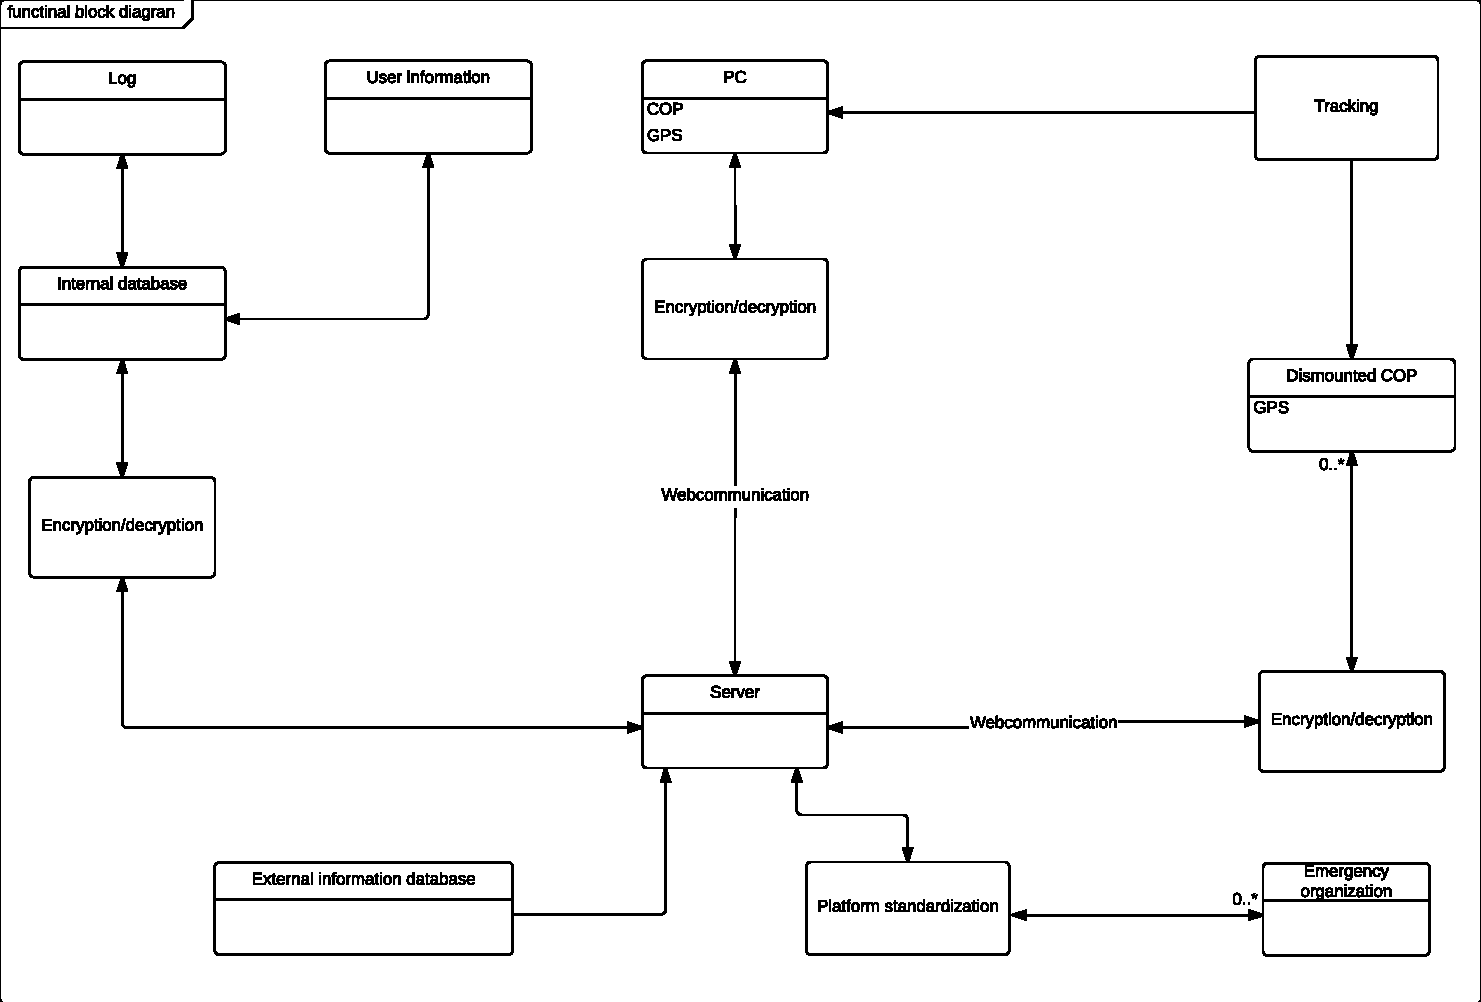
\includegraphics[width=0.95\textwidth]
{billeder/functional_block_diagram.pdf}
\caption{Functional block diagram of the system.}
\label{fig:func_block_diagram}
\end{figure}

The diagram consists of system-blocks and function-blocks. The system-blocks are depicted as two-compartment blocks with the name of the block in the first compartment, and sub parts in the second compartment. The functions are blocks with a single compartment, containing the name of the function. The system-blocks are actual parts of the system, while the function-blocks are functions and actions that are carried out in the system. The data flow between the blocks are depicted with arrows, whose direction dictates the direction of the data flow. 

\subsubsection{Block description}
In this section a short description of each system- and function-block is given.

\textbf{System-blocks}
\begin{enumerate}
\item[•] \textbf{PC:} This block constitutes the machine in the head quarter (HQ) on which the COP-software will be executed. It also has a GPS module, so that the location of the HQ is always known. The PC is to be connected to the internet, in order to be able to communicate with the rest of the system.
\item[•] \textbf{Server:} The server will facilitate communication between the other blocks. In addition, it will store user information along with logs locally in an internal database.
\item[•] \textbf{Log:} The log will contain log entries with information about previous events.
\item[•] \textbf{User information:} This block will contain information about the users of the system.
\item[•] \textbf{Internal database:} The internal database will be responsible for storing the log and user information.
\item[•] \textbf{External information database:} This block constitutes the source of static and dynamic information, that the COP will make available to the user.
\item[•] \textbf{Dismounted COP:} This block constitutes the machine on which the condensed COP-software will be executed. The dismounted COP will be used by the dismounted users in the field. It has a GPS module, so that the location of the dismounted users is always known. Furthermore it has a GSM module so that it will be able to communicate with the rest of the system.
\item[•] \textbf{Emergency organization:} These blocks constitute the platforms currently employed by the various emergency organizations using the system.
\end{enumerate}


\textbf{Function-blocks}
\begin{enumerate}
\item[•] \textbf{Encryption/decryption:} These blocks will be responsible for encrypting outgoing data and decrypting incoming data in the communication between the various system blocks.
\item[•] \textbf{Tracking:} This block constitutes all communication with GPS-satellites.
\item[•] \textbf{Platform standardization:} This block is responsible for unifying all communication between the various emergency organizations using the system, and the COP/dismounted COP.
\end{enumerate}

\subsection{State machine diagram}
The the state machine diagram is shown in figure \ref{fig:state_diagram}:

\begin{figure}[H]
\centering
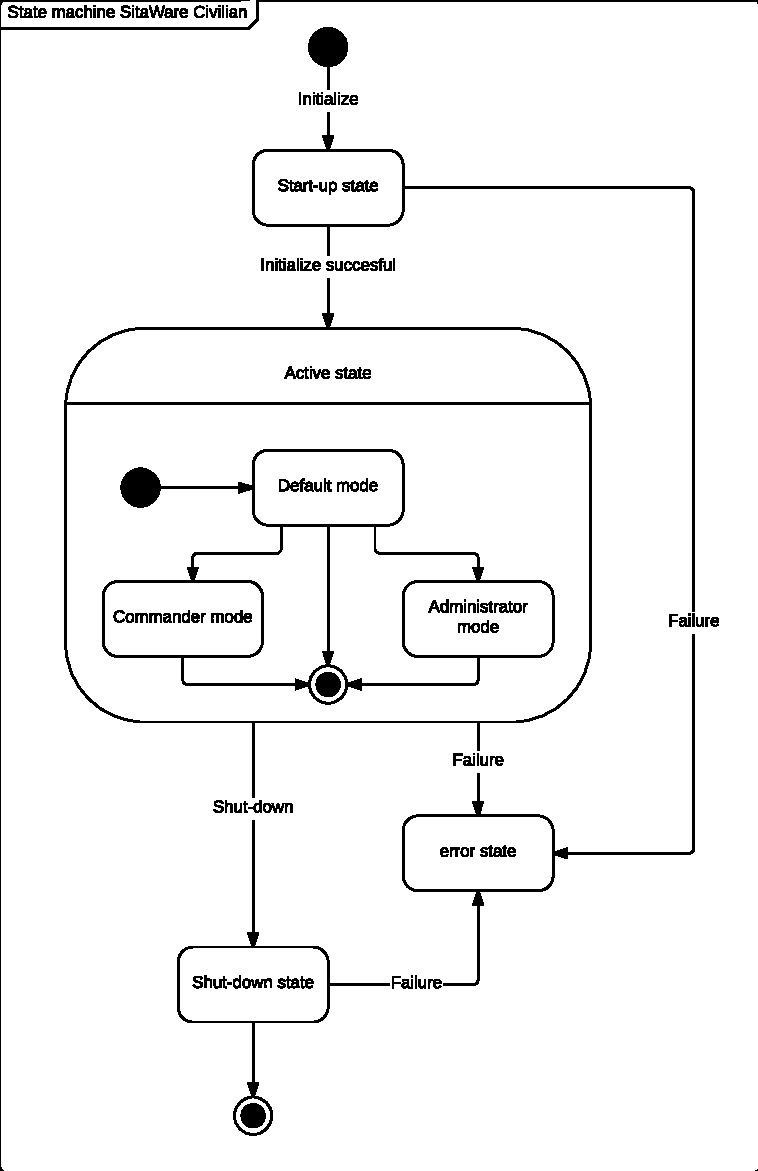
\includegraphics[width=0.95\textwidth]
{billeder/state_machine_pdd.pdf}
\caption{State machine diagram of the system.}
\label{fig:state_diagram}
\end{figure}

In accordance with the System Requirement Specification, the system has four states: a start-up state, an active state, an error-state and a shut-down state. When in the active state, the system can operate in three different modes. If an error occurs anywhere in the start-up, active or shut-down state, the system will enter an error state, where the error can be remedied.
%Referenced documents
\chapter{Referenced Documents}
This chapter contains a brief description of the documents referenced to in this document.

\begin{table}[H]  
\centering
\scalebox{1.0}{
\begin{tabular}{|l|l|p{6cm}|}
\multicolumn{3}{l}{}\\\hline
	\textbf{Version}	&\textbf{Document name}		&\textbf{Description}		\\\hline
	\textbf{1.3}		& System Requirement Specification		& The System Requirement Specification(SRS) contains all of the requirements that the system has to fulfil. 		\\\hline

\end{tabular}}
\caption {Referenced Documents.} 
\label{tab:table_ReferencedDocuments} 
\end{table} 

%%%% Fixme-listen %%%%
%\newpage										% Ny side til Fixme-listen
%\listoffixmes									% Fixme-listen - fjernes til sidst i projektet med "%"



\end{document}									% Slutter dokumentet - obligatorisk